\documentclass[11pt,a4paper]{article}
\usepackage[utf8]{inputenc}
\usepackage[french]{babel}
\usepackage[T1]{fontenc}

\usepackage{amsmath}
\usepackage{amsfonts}
\usepackage{amssymb}

\newcommand{\NomAuteur}{Fabrice BOISSIER}
\newcommand{\TitreMatiere}{Algo et Structure de Données 1}
\newcommand{\NomUniv}{EPITA - Bachelor Cyber Sécurité}
\newcommand{\NiveauUniv}{CYBER1}
\newcommand{\NumGroupe}{CYBER1}
\newcommand{\AnneeUniv}{2022-2023}
\newcommand{\DateExam}{Octobre 2022}
\newcommand{\TypeExam}{QCM 1}
\newcommand{\TitreExam}{\TitreMatiere}
\newcommand{\DureeExam}{20 min}
\newcommand{\MyWaterMark}{\AnneeUniv} % Watermark de protection

% Ajout de mes classes & definitions
\usepackage{MetalExam} % Appelle un .sty

% "Tableau" et pas "Table"
\addto\captionsfrench{\def\tablename{Tableau}}

%%%%%%%%%%%%%%%%%%%%%%%
%Header
%%%%%%%%%%%%%%%%%%%%%%%
\lhead{\TypeExam}							%Gauche Haut
\chead{\NomUniv}							%Centre Haut
\rhead{\NumGroupe}							%Droite Haut
\lfoot{\DateExam}							%Gauche Bas
\cfoot{\thepage{} / \pageref*{LastPage}}	%Centre Bas
\rfoot{\texttt{\TitreMatiere}}				%Droite Bas

%%%%%

\usepackage{tabularx}

\newlength{\LabelWidth}%
%\setlength{\LabelWidth}{1.3in}%
\setlength{\LabelWidth}{1cm}%
%\settowidth{\LabelWidth}{Employee E-mail:}%  Specify the widest text here.

% Optional first parameter here specifies the alignment of
% the text within the \makebox.  Default is [l] for left
% alignment. Other options are [r] and [c] for right and center
\newcommand*{\AdjustSize}[2][l]{\makebox[\LabelWidth][#1]{#2}}%


\definecolor{mGreen}{rgb}{0,0.6,0}
\definecolor{mGray}{rgb}{0.5,0.5,0.5}
\definecolor{mPurple}{rgb}{0.58,0,0.82}
\definecolor{backgroundColour}{rgb}{0.95,0.95,0.92}

\lstdefinestyle{CStyle}{
    backgroundcolor=\color{backgroundColour},
    commentstyle=\color{mGreen},
    keywordstyle=\color{magenta},
    numberstyle=\tiny\color{mGray},
    stringstyle=\color{mPurple},
    basicstyle=\footnotesize,
    breakatwhitespace=false,
    breaklines=true,
    captionpos=b,
    keepspaces=true,
    numbers=left,
    numbersep=5pt,
    showspaces=false,
    showstringspaces=false,
    showtabs=false,
    tabsize=2,
    language=C
}


\hyphenation{op-tical net-works SIGKILL}


\begin{document}

% \MakeExamTitleDuree     % Pour afficher la duree
\MakeExamTitle                   % Ne pas afficher la duree

%% \MakeStudentName    %% A reutiliser sur chaque nouvelle page


% \setcounter{section}{1}  % Ne pas faire une liste de 0.1, 0.2, ... mais 1.1, 1.2, ...

\renewcommand{\thesubsection}{\arabic{subsection}} % Subsection sans 0.x, mais juste x

% \newcommand{\thesubsection}{\thesection.\arabic{subsection}} % Subsection avec numero section (0.x)


\vfillFirst

\subsection{(4 points) Quels éléments affichés dans l'image sont absents de la structure associée ? }

\begin{table}[h!]
  \centering
  \begin{minipage}{0.4\textwidth}
    \centering
% %*   *)
\begin{lstlisting}[style=algorithmique]
struct player
  enum action cur_action
  enum action prev_action
  int  HP
  int  lifes
  int  speed
  int  time
  int  pos_x
  int  pos_y
fin struct \end{lstlisting}
    % \caption{Algorithme de la somme des N premiers entiers}
    % \label{algo-somme-n-premiers-entiers}
  \end{minipage}
  \hfillx
  \begin{minipage}{0.55\textwidth}
    \centering
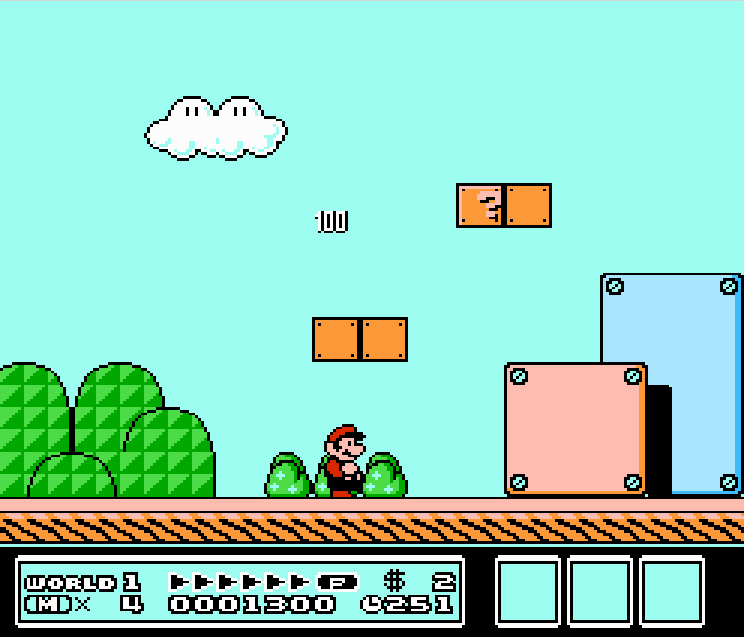
\includegraphics[width=\textwidth]{img/mario3.png}
  \end{minipage}
%  \caption{Algorithme de la somme des N premiers entiers}
%  \label{somme-n-premiers-entiers}
\end{table}

\begin{itemize}
  \item[\CaseCoche] Points de vie/Taille de Mario \\
  \item[\CaseCoche] Score \\
  \item[\CaseCoche] Pièces/Argent \\
  \item[\CaseCoche] Monde \\
  \item[\CaseCoche] Vies \\
\end{itemize}


\bigskip
\vspace*{1cm}


\subsection{(4 points) Cochez la (ou les) affirmation(s) vraie(s) : \og Un pointeur est... \fg }

\begin{itemize}
  \item[\CaseCoche] Une structure \\
  \item[\CaseCoche] Une instruction \\
  \item[\CaseCoche] Une référence vers le contenu d'une variable \\
  \item[\CaseCoche] L'adresse d'une case en mémoire \\
\end{itemize}


\vfillLast

%\bigskip
\newpage

\vfillFirst


\subsection{(4 points) Si l'on déréférence un pointeur, on peut trouver au bout : }

\begin{itemize}
  \item[\CaseCoche] Une unique valeur \\
  \item[\CaseCoche] Un tableau de plusieurs valeurs de même type côte à côte \\
  \item[\CaseCoche] Une structure de données contenant un ou plusieurs champs \\
  \item[\CaseCoche] Un blocage de l'accès avec une erreur car on n'aurait pas du accéder à cette adresse \\
  \item[\CaseCoche] Une adresse vers une autre case mémoire \\
\end{itemize}


\bigskip
\vspace*{1cm}


\subsection{(4 points) Cochez la (ou les) affirmation(s) vraie(s) : }

\begin{center}
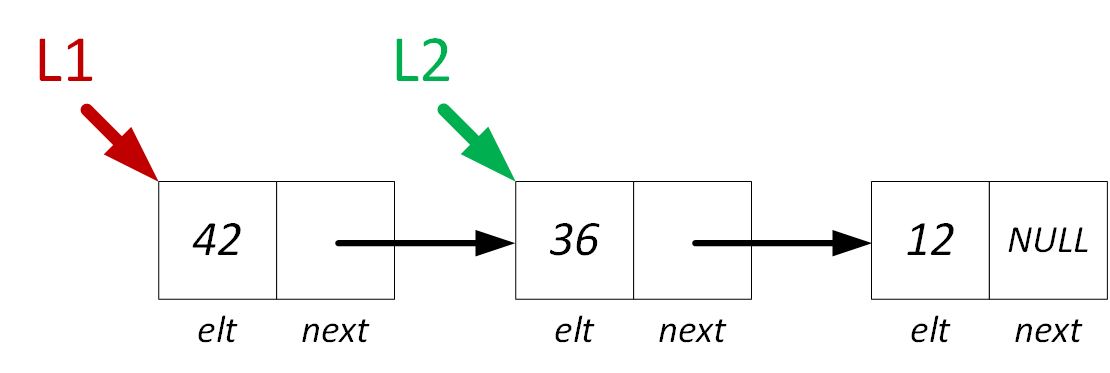
\includegraphics[width=0.75\textwidth]{img/liste1.png}
\end{center}

\begin{itemize}
  \item[\CaseCoche] \lstinline[style=algorithmique]! L1 == L2 ! \\
  \item[\CaseCoche] \lstinline[style=algorithmique]! (*L1) == (*L2) ! \\
  \item[\CaseCoche] \lstinline[style=algorithmique]! (*L1).next == L2 ! \\
  \item[\CaseCoche] \lstinline[style=algorithmique]! (*L1).next == (*L2) ! \\
  \item[\CaseCoche] \lstinline[style=algorithmique]! (*(*L1).next) == (*L2) ! \\
  \item[\CaseCoche] \lstinline[style=algorithmique]! (*(*L1).next) == L2 ! \\
\end{itemize}


\vfillLast

%\bigskip
\newpage

\subsection{(4 points) Cochez la (ou les) affirmation(s) vraie(s) : }

\begin{lstlisting}[style=algorithmique]
variables
  int **i
  int *j
  int k

i = allouer(taille(int*))
j = allouer(taille(int))
k = 0
i = &j
(*j) = k
k = 42
\end{lstlisting}

\begin{itemize}
  \item[\CaseCoche] \lstinline[style=algorithmique]! i == 42 ! \\
  \item[\CaseCoche] \lstinline[style=algorithmique]! (*i) == 42 ! \\
  \item[\CaseCoche] \lstinline[style=algorithmique]! (*(*i)) == 42 ! \\
  \item[\CaseCoche] \lstinline[style=algorithmique]! i == 0 ! \\
  \item[\CaseCoche] \lstinline[style=algorithmique]! (*i) == 0 ! \\
  \item[\CaseCoche] \lstinline[style=algorithmique]! (*(*i)) == 0 ! \\
\end{itemize}


\bigskip


\subsection{[BONUS] (0 point) Parmi les personnages "François Pignon" créés par Francis Veber... }

\begin{itemize}
  \item[\CaseCoche] un a travaillé au ministère des finances \\ % Pignon : Dîner de cons
  \item[\CaseCoche] un était représentant en chemises \\ % Pignon : L'Emmerdeur
  \item[\CaseCoche] un était violoniste \\ % Perrin : Le Grand Blond avec une chaussure noire
  \item[\CaseCoche] un voulait ouvrir un bistrot "Aux deux amis" \\ % Quentin : Tais-toi !
  \item[\CaseCoche] un était comptable \\ % Perrin : La Chèvre
\end{itemize}

\end{document}
